\documentclass{school-22.101-notes}
\date{November 2, 2011}

\begin{document}
\maketitle



%%%%%%%%%%%%%%%%%%%% Nuclear Shell Model %%%%%%%%%%%%%%%%%%%%%%%%%%%%%%%%%%%%%%%
\lecture{Nuclear Structure}
While we can always do more scattering experiment, it is easier and more interesting to do an over simplified theory, the shell model, of which we can extract many microscopic description of properties. The shell model is analogous to the electronic structure of an atom, in that we fill shells with electrons as energy increases, while taking into account Pauli exclusive principle. Refer to Krane 5.1, 5.2 and Meyerhof 2.5. 

There are a couple of assumptions/properties for shell model: 
\begin{itemize}
\item In nuclei there are protons and neutrons;
\item Each particle group is separately distributed over certain energy states, subject to the Pauli exclusive principle;
\item Nuclei also have excited states;
\item Nucleons can be added or removed from a nucleus. 
\end{itemize}

\uline{Atomic Physics vs. Nuclear Physics}
Atomic physics is relatively easy because you have one particle (electron) sitting in an external potential that we can solve for analytically; whereas nuclear physics deals with particles (neutron, photons etc) sitting in a self-generated potential that there are no easy analytical solutions. 
\begin{table}[h!]
    \centering
    \begin{tabular}{|c|c|c|} \hline
    & Atomic Physics & Nuclear Physics \\ \hline
    Type(s) of Particles &   1: $e^-$ (subject to Pauli Exclusive Principle) & 2: $n, p$ \\ \hline
    Governing Potential & Coulomb potential & Strong force potential \\ \hline
    Potential Property & $V(r)$ is external to $e^-$ & $V(r)$ is self-generated by $n,p$ \\ \hline
    \end{tabular}
    \caption{Comparison of Atomic Physics and Nuclear Physics}
\end{table}

Structure of nucleus is more complex than the electronic structure of atoms because there is no center of attraction anymore; nucleons are held together by their mutual interactions which are more complicated than Coulomb force. 


\topic{Overview}
\begin{enumerate}
\item \textbf{Liquid Drop Model}. So far we have considered deuteron, which contains two particles. In this section we will consider heavier nuclei with multiple nucleons. Moving from two body problem to many body problem sounds hard, though thanks to the \textit{paring effect}, we do not have to study every nucleon; it's the last one or two nucleon that matters. We consider the `liquid drop' model, that is, we assume neutrons and protons to be in a homogeneous `soup.' 

\item \textbf{SEMF}. The liquid drop model leads to the SEMF, which is a smooth curve; but we know from observations, there are isotopes diverse from the smooth curve in a pattern (i.e., the nuclide with magic numbers). See Section~\ref{magic-number}.


\item \textbf{Intermediate Potential}. We consider the potential: The two extreme forms as seen in Fig.~\ref{potential-candidates} are, when $R \to 0$ we get a harmonic oscillator potential, and when $a \to 0$ we get a square well. The real potential is somewhere between the two models. That's why we need the intermediate potential model. See Section~\ref{candidate-potentials}.
\begin{figure}[ht]
  \centering
  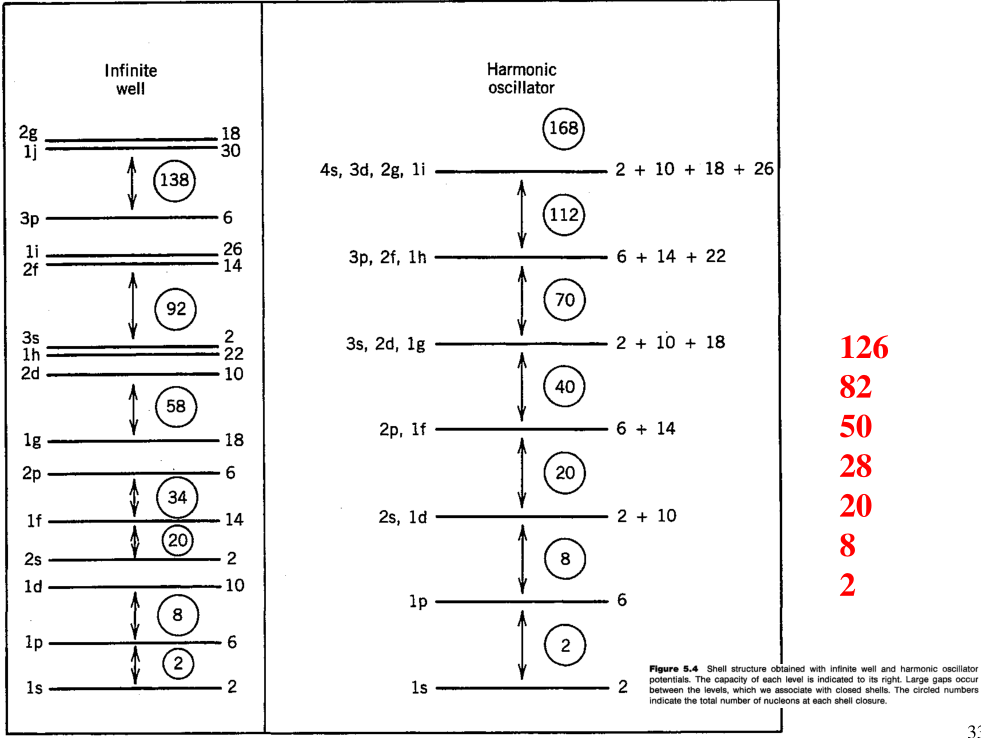
\includegraphics[width=5in]{images/ns/potential-candidates.png}
  \caption{Two Potentials for Describing Nuclear Structure} \label{potential-candidates}
\end{figure}

\item \textbf{Spin Orbital Coupling}. To capture the magic numbers, we consider the orbital-spin coupling. $I = j_i$ where $i$ is the singlet of the last nucleon. $j_i = l_i + s_i = l\pm \frac{1}{2}$, that is, we get degeneracy.  We can either consider the modified potential $V_{so} \to V_{so} (l \cdot s)$  or we can consider the modified energy: 
\eqn{ E_{j_i = l_i + 1/2} - E_{j_i = l_i - 1/2} = \expect{ \frac{ \left( l_i + \frac{1}{2} \right) \left( l_i + \frac{3}{2} \right) - \left( l_i - \frac{1}{2} \right) \left( l_i + \frac{1}{2} \right) }{2} V_{so} (r) } = \left( l_i + \frac{1}{2} \right) V_{so} (r) < 0  }
If we add the spin orbit dependence onto the intermediate form, we get a form close to observations. See Section.~\ref{spin-orbit-coupling}. 
\end{enumerate}




\topic{Evidence for Magic Number and Shell Model} \label{magic-number}
Each shell is filled with a given number of nucleons of each kind. Experiments indicate special features of the number of nucleons at the these `Nuclear Magic Numbers' (Z or N): 2, 8, 20, 28, 50, 82, 126 \footnote{For heavier undiscovered nuclei, N: $184, 196, 272, 318, \cdots$ Z: $114, 126, 164, \cdots$}. Nuclei with magic number of neutron or proton or both are very stable. Notice atomic magic numbers are different from nuclear magic numbers; they are: 2, 10, 18, 30, 36, 48, 54, ...

Evidence for magic number and the shell model:
\begin{enumerate}
\item Abundance of stable isotones (Isotones: same neutron number N, but different proton number Z; Isotopes: same proton number Z, but different neutron number N) is large (by 5 to 7 times) for nuclei with magic number of neutrons.
\begin{figure}[ht]
    \centering
    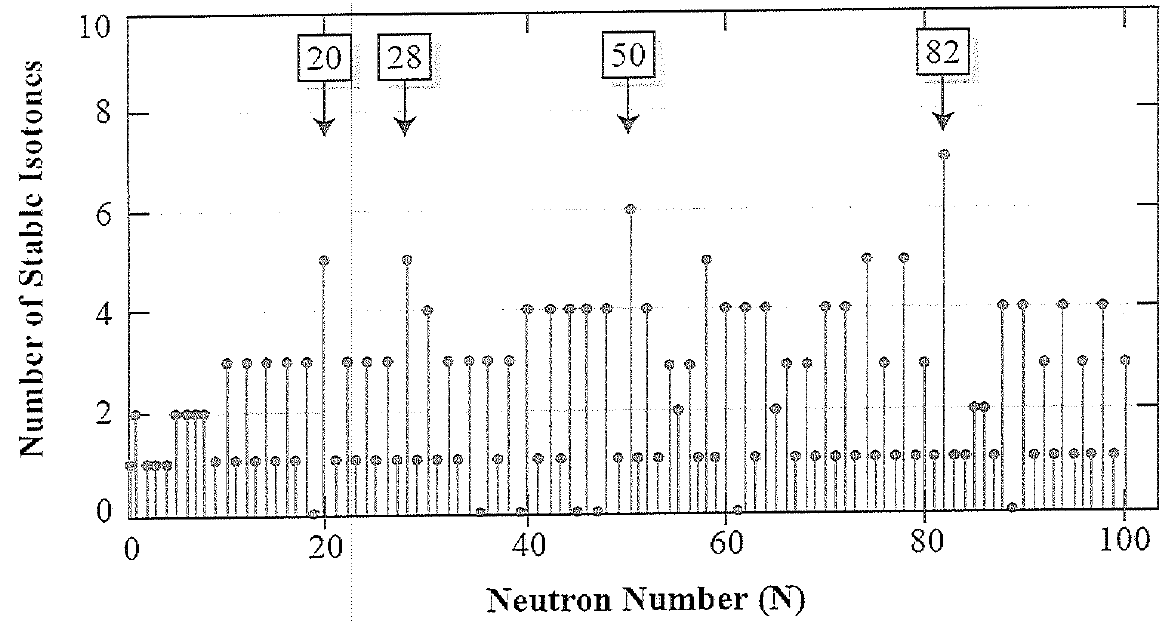
\includegraphics[width=3in]{images/shell/shell-evidence-1.png}
    \caption{Shell Model Evidence 1: Histogram of Stable Isotones Showing Nuclides with Magic Numbers Are More Abundant}
\end{figure}
\item Neutron separation energy $S_n$ is low for nuclei with one more neutron than a magic number. Reason: it is easier to separate one neutron when number of neutrons is magic plus 1; that is, magic neutron numbers are more tightly bound \footnote{Also see Krane Figure 5.2}. 
\begin{figure}[ht]
    \centering
    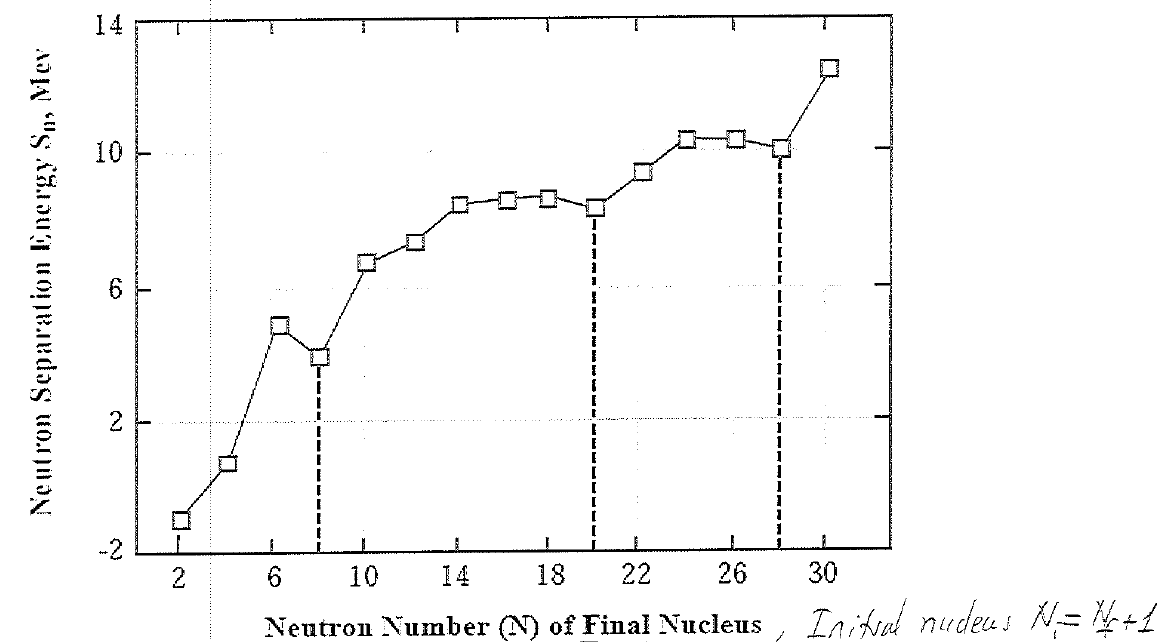
\includegraphics[width=3in]{images/shell/shell-evidence-2.png}
    \caption{Shell Model Evidence 2: Neutron Separation Energy as a Function of Neutron Number N}
\end{figure}
\item The first excited states of even-even nuclei (meaning even neutron, even proton) have higher than usual energies at magic numbers because, again, these nuclei are tightly bound. Excite states mean take one or more nuclei to a higher state to break the bound energy. If tightly bound, then excite energy increases. 
\begin{figure}
    \centering
    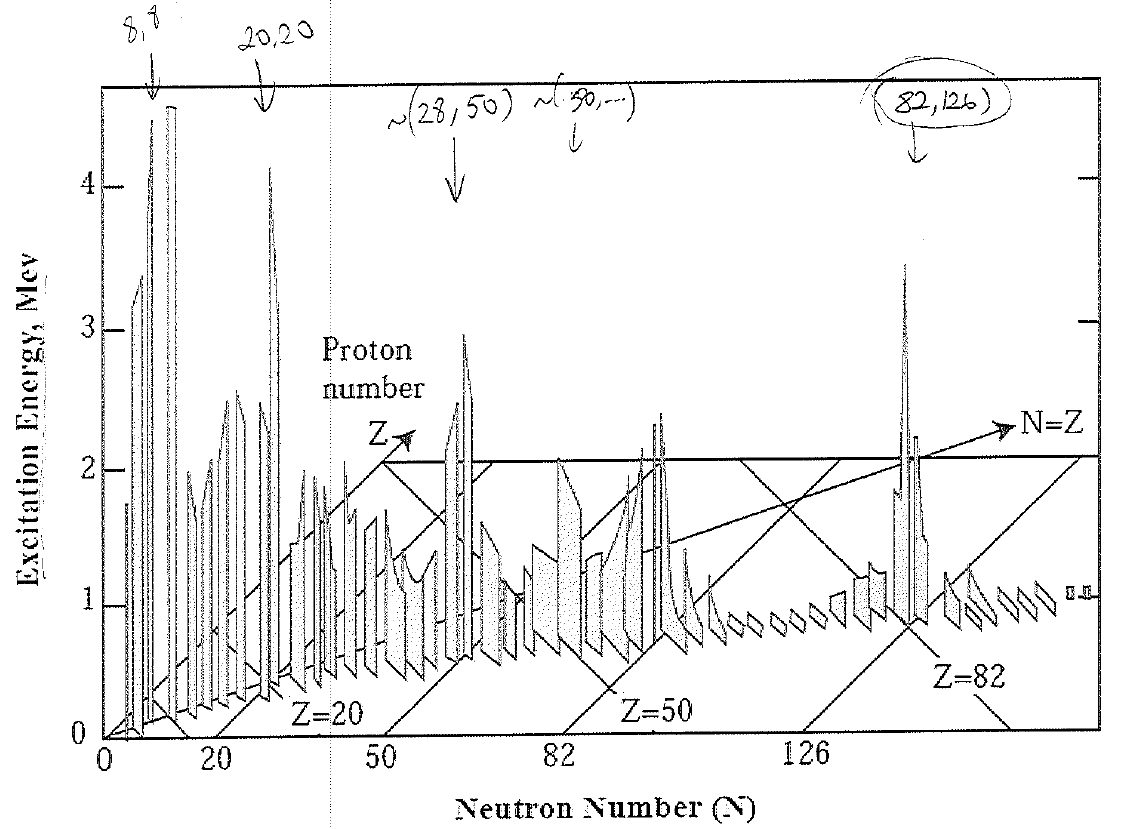
\includegraphics[width=3in]{images/shell/shell-evidence-3.png}
    \caption{Shell Model Evidence 3: First Excited States of Even-Even Nuclei Are Higher Than Usual Energies}
\end{figure}
\item Neutron capture cross sections are low for these numbers: they are stable already, do not want to absorb neutron. Zr has Z=40 and has about 50,51,52 neutrons, hence it is `neutron transparent.'
\begin{figure}
    \centering
    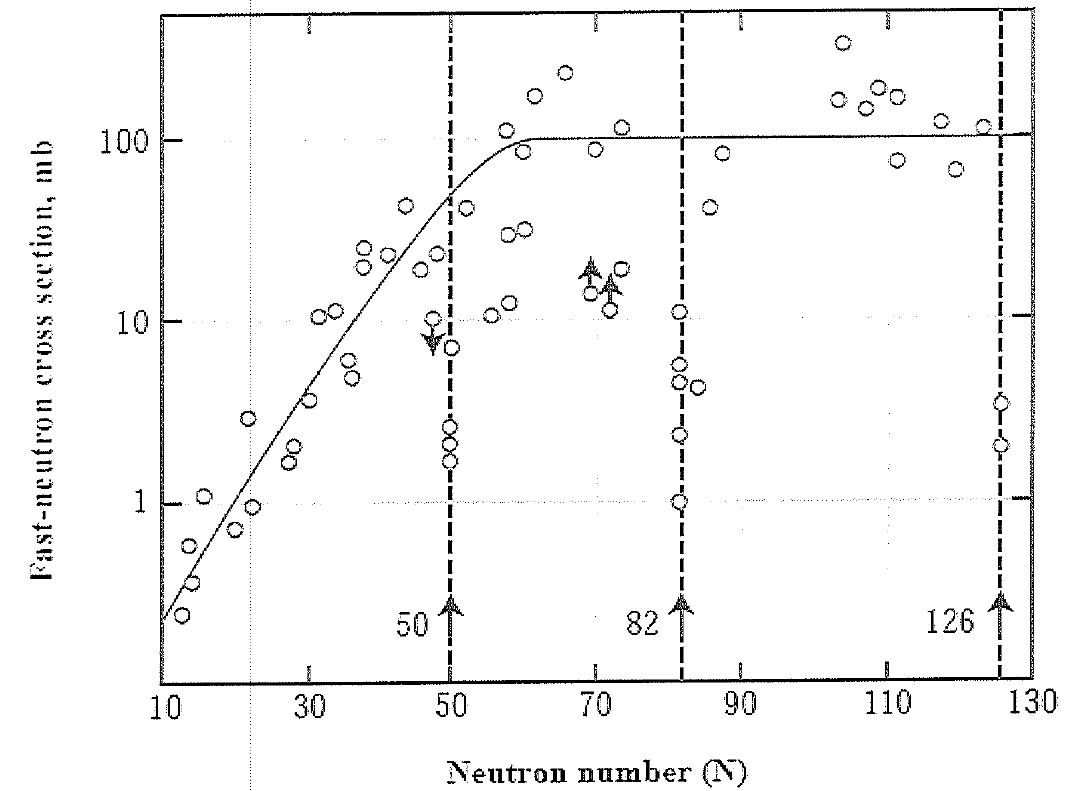
\includegraphics[width=3in]{images/shell/shell-evidence-4.png}
    \caption{Shell Model Evidence 4: Neutron Capture Cross-sections are Lower}
\end{figure}
\item Nuclear charge radius decreases and then suddenly jumps at magic numbers. 
\begin{figure}
    \centering
    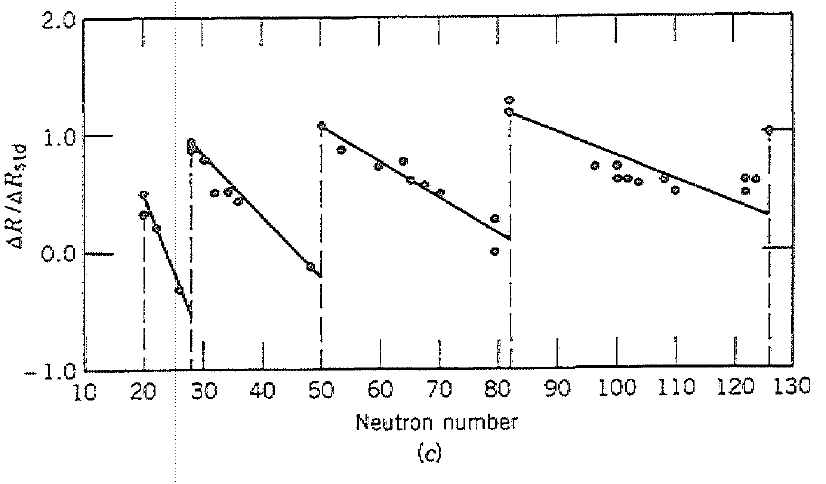
\includegraphics[width=3in]{images/shell/shell-evidence-5.png}
    \caption{Shell Model Evidence 5: Neutron Charge Radius Jumps at Magic Numbers}
\end{figure}
\end{enumerate}






\topic{Many-Body Hamiltonian} 
We are going to make the ``independent particle assumptions" which enable us to replace an n-body problem with n single-body problem:
\eqn{ \Hhat \approx \Sum_i \Hhat_i }
The independent particle assumption comes from ignoring the residual interaction terms: 
\begin{align}
 \Hhat &= \overbrace{\Sum_i \frac{\phat^2_i}{2m_i}}^{\mathrm{KE}} + \overbrace{\Sum_{i \le j} V(|x_i - x_j|)}^{\mathrm{Strong \fsp Force}} + \overbrace{\Sum_{i \le j} \frac{e^2}{|x_i - x_j|}}^{\mathrm{Coulomb, \fsp for \fsp p \fsp only}} \\
 &= \underbrace{ \Sum_i \left[ \frac{\phat^2_i}{2m_i} + V_{\mathrm{nuc}} (|x_i|) + V_{\mathrm{Coul}} (|x_i|)  \right]}_{\mbox{mean field}}  + \underbrace{\Sum_{i \le j} V(|x_i - x_j|) - \Sum V_{\mathrm{nuc}} (|x_i|) + \Sum V_{\mathrm{Coul}} (|x_i - x_j|) - \Sum V_{\mathrm{Coul}} (|x_i|) }_{\mbox{residual interactions from inter-nucleon couplings} } \\
 &= \Sum_i \Hhat_i + \underbrace{\Hhat_{\mbox{residual interaction}}}_{\to 0} \approx \Sum_i \Hhat_i \\
\Hhat_i &= \frac{\phat^2_i}{2m_i} + V_{\mathrm{nuc}} (|x_i|) + V_{\mathrm{Coul}} (|x_i|) 
\end{align}
Implications from the above derivation:
\begin{itemize}
\item Gaussian unit is used (so no $\frac{1}{4 \pi \epsilon}$ anymore); 
\item This assumption is for a independent particle single nucleon (n or p) moving in a force field ( nuclear plus coulomb) that is generated by all other nucleons; 
\item While there is strong interactions between nucleons, motion of each nucleon is practically independent of any other nucleon; 
\item $V_{\mathrm{Coul}} (|x_i|)$ term exists for protons only; 
\item Potential terms ($V_{\mathrm{nuc}} (|x_i|), V_{\mathrm{Coul}} (|x_i|)$) need to be modeled; choice of potential is important in predictions (see next section).
\end{itemize}

To model the potential, we will consider the following common ones: 
\begin{enumerate}
\item Infinite Well. It does not work because it requires infinite amount of energy to separate a $n$ or $p$; model has sharp edge, whereas nuclear charge and matter distribution fall smoothly to zero beyond the mean radius.
\item Harmonic Oscillator: the potential is parabolic. It does not work because the energy goes to infinity, and the potential inside of the well is not sharp enough (compare with experimental results); its advantage is that it allows analytical solution;
\item Intermediate Potential: somewhat like a finite potential well (has a region of -$V_0$), but the edge is smooth. 
\end{enumerate}

%%%%%%%%%%%%%%% Harmonic Oscillator %%%%%%%%%%%%
\topic{Potential Models} \label{candidate-potentials}
\subtopic{Harmonic Oscillator Potential: Derivations}
We define the potential well as a parabolic well from $-R_0$ to $R_0$ with a maximum depth of $-V_0$: 
\begin{align}
V_{\mathrm{nuc}} (r) &\approx - V_0 \left( 1 - \frac{r^2}{R_0^2} \right) = \frac{V_0}{R_0^2} (r^2 - R_0^2)  \\
V_{\mathrm{Coul}} (r) &= \frac{(Z-1) e^2}{R_0} \left[ \frac{3}{2} - \frac{1}{2}  \frac{r^2}{R_0^2}\right] 
\end{align}
Notice, again, $V_{\mathrm{Coul}}$ is only a concern for the protons; for constant proton density inside the nucleus, coulomb field is parabolic, though as $r > R_0$, real coulomb potential remains positive (and small), while the parabolic model goes to negative: 

\begin{figure}[h!]
    \centering
    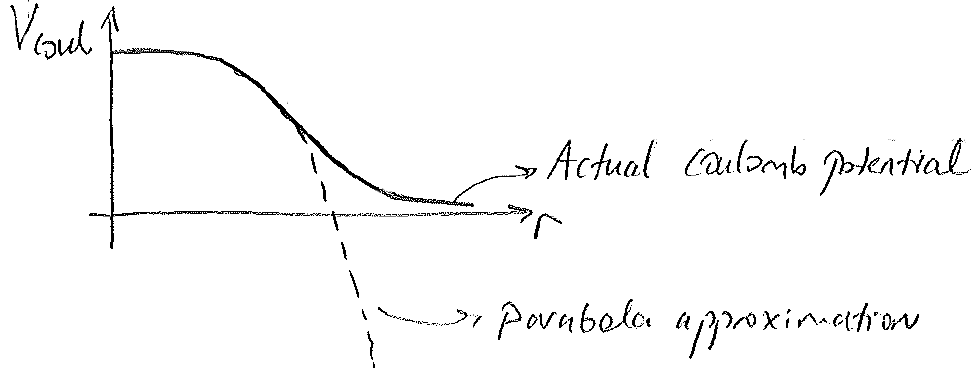
\includegraphics[width=3in]{images/shell/Vcoul-parabolic-model.png}
    \caption{Actual Coulomb Potential vs. Its Parabolic Approximation}
\end{figure}

\begin{align}
V_{\mathrm{eff}} (r) = 
\begin{dcases*}
V_{\mathrm{nuc}}  = \frac{V_0}{R_0^2} r^2 - V_0 
& neutrons (deeper,narrower well) \\
V_{\mathrm{nuc}} + V_{\mathrm{Coul}} = \overbrace{ r^2 \left[ \frac{V_0}{R_0^2} - \frac{(Z_1)e^2}{2 R_0^3} \right] }^{\frac{1}{2} m \omega^2 r^2} - \overbrace{ \left[  V_0 - \frac{3}{2} \frac{(Z-1) e^2}{R_0} \right] }^{V_0^{\prime} }   & protons (shallower,wider well) 
\end{dcases*}
\end{align}

From the above discussion, we can see that $V_{\mathrm{eff}}$ takes the general form of $\boxed{V_{\mathrm{eff}} = \frac{1}{2} m \omega^2 r^2 - V_0^{\prime}},$ 
\begin{align}
\omega^2 =
\begin{dcases*}
\frac{2}{m} \frac{V_0}{R_0^2}  & neutrons \\
\frac{2}{m} \left[ \frac{V_0}{R_0^2} - \frac{(Z-1) e^2}{2 R_0^3} \right] & protons \\
\end{dcases*}
\fsp \fsp \fsp \fsp \fsp
V_0^{\prime} = 
\begin{dcases*}
V_0 & neutrons \\
V_0 - \frac{3}{2} \frac{(Z-1) e^2}{R_0} & protons \\
\end{dcases*}
\end{align}


\subtopic{Harmonic Oscillator Potential: Solutions}
Since the potential is a central potential, the angular part of the solution to the Schrodinger equation is just $Y_{ml} (\theta, \phi)$ \footnote{The angular part to any central potential is harmonic oscillator}. The radial part for the 1D case can be expressed as the product of a finite polynomial and an exponential: 
\eqn{\psi (r) =   \mbox{polynomials (n,l ) } \times \exp\left( - \frac{\alpha^2 r^2}{2} \right) }
Some sample radial wavefunctions for 3D SHO problem can be found in Table~\ref{radial-wavefunction-SHO}. 

\begin{table}[h!]
    \centering
    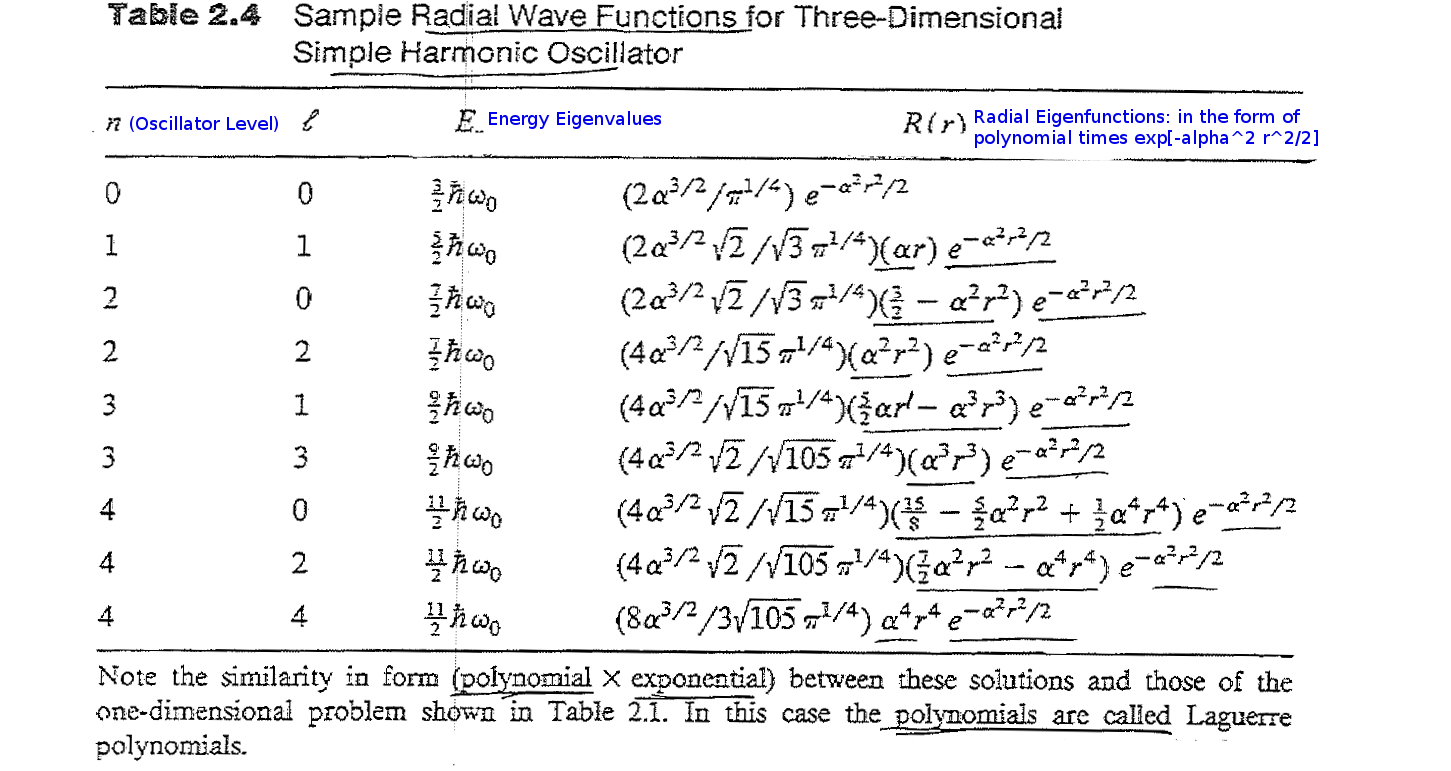
\includegraphics[width=6in]{images/shell/radial-wavefunction-SHO.png}
    \caption{Sample Radial Wave Functions for 3D Simple Harmonic Oscillator (Table 2.4, Krane)}
    \label{radial-wavefunction-SHO}
\end{table}

Harmonic Oscillator Energy Eigenvalues \footnote{See Liboff for details. $\frac{3}{2}$ is for 3D, it would be replaced by $\frac{1}{2}$ if we are discussing 1D}: 
\eqn{ E_n = \hbar \omega \left( n + \frac{3}{2} \right) - V_0^{\prime}  }
It is important to notice that energy does not depend on $l, m_l$, and not all values of $l$ are permitted for each $n$. From mathematical solution of the radial equation, the allowed quantum numbers: 
\begin{enumerate}
\item Given the Oscillator Level $n$, $l$ has to satisfy:
\eqn{ l \le n, \mbox{if n is even, then l has to be even; n is odd, l has to be odd.} }
\item Knowing $l$, $-l \le m_l \le l$, hence $2l+1$ degeneracy, also take into account $m_s = \pm \frac{1}{2}$, then the total degeneracy is \eqn{ D_l (l) = 2l+1, \fsp D_{l,s} (l) = 2(2l+1) = 4l+2 }
\item Written $D_{l,s}$ as a function of $n$, the total number of degeneracy is: 
\eqn{ D_l (n) = \frac{1}{2} (n+1)(n+2), \fsp D_{l,s} (n) = (n+1)(n+2) }
\end{enumerate}

Example: given $n =5$, $l = 1,3,5$. Then $ m_l = \pm 1, 0 (3); \pm 3, \pm 2, \pm 1, 0 (7); \pm 5, \pm 4, \pm 3, \pm 2, \pm 1, 0 (11)$. Together that is 21 degeneracy. Also take into account the 2 degeneracy of $m_s$, then in total there is 42 degeneracy. Notice this agrees with $D_n = (n+1)(n+2) = 42$. Table~\ref{energy-SHO} lists some lower energy levels \footnote{Spectroscopic Notation: $l=0 (s), l=1 (p), l=2 (d), l=3 (f), l=4 (g), l=5(h), l=6 (i), l=7(k), l=8(l), \cdots$. The letter is only associated with $l$ value, and the number distinguish this $(n,l)$ combination with a previous one}:  
\begin{table}[h!]
    \centering
    \begin{tabular}{|c|c|c|c|c|c|} \hline
    n & Energy $\frac{V_0 + E }{\hbar \omega_0}$ & states $(n,l)$ & Spectroscopic Notation & $D_{l,s} (n)$  & Cumulation $ \left( \Sum_n D_n \right)$ \\ \hline 
    0 & $3/2$ & (0,0) & 1s & 2 & 2 \\ \hline
    1 & $5/2$ & (1,1) & 1p & 6 & 8\\ \hline
    2 & $7/2$ & (2,0), (2,2) & 2s, 1d & 12 & 20 \\ \hline
    3 & $9/2$ & (3,1), (3,3) & 2p, 1f & 20 & 40 \\ \hline
    4 & $11/2$ & (4,0), (4,2), (4,4) & 3s, 2d, 1f & 30 & 70 \\ \hline
    \end{tabular}
    \caption{Lower Energy Levels of A Particle in a Central 3D Simple Harmonic Oscillator}
    \label{energy-SHO}
\end{table} 

Two issues with the harmonic oscillator model:  
\begin{enumerate}
\item The total number of allowed energies are correct for $n = 0,1,2$, but off for higher magic numbers.  
\item The separation energy:  
\eqn{ \Delta E = \hbar \omega \left[ \left( n + 1 + \frac{3}{2} \right) - \left( n + \frac{3}{2} \right) \right] = \hbar \omega = \hbar \sqrt{\frac{2V_0}{m R_0^2} - \frac{(Z-1) e^2}{R_0^3} }  }
For neutrons, if we plug in $R_0 = 1.25 A^{1/3} \fsp \fm$, and get ride of the coulomb term, then $V_0 \approx 50 A^{-1/3} \MeV$. We notice as A increases, $\Delta E $ approaches 10 MeV. That is to say, for a typical well depth of 50 MeV, we can fit around 4 oscillator energy levels in it, which does not agree with reality\footnote{there are clearly A's that have more than 4 possible energy levels.}. Notice the above discussion is for neutrons. The energy levels are shifted up for protons. 
\end{enumerate}


%%%%%%%%%%%%%%%% Intermediate Potentials %%%%%%%%%%%%%
\subtopic{Intermediate Potential}
\begin{figure}[h!]
    \centering
    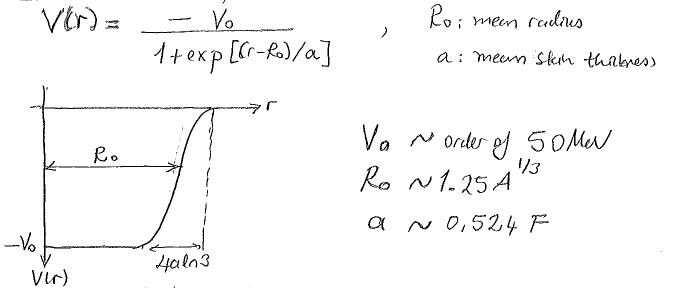
\includegraphics[width=4in]{images/shell/intermediate-form-potential.png}
    \caption{Intermediate Form Potential Diagram}
\end{figure}

It is more representative of strong potential, with sufficiently sharp edge, and sufficiently smooth decay to reach zero around $R_0$. As seen in Figure~\ref{intermediate-energy}, again magical number 2,8, 20 are predicted correctly, but higher shell occupancy numbers are off. 

\begin{figure}[h!]
    \centering
    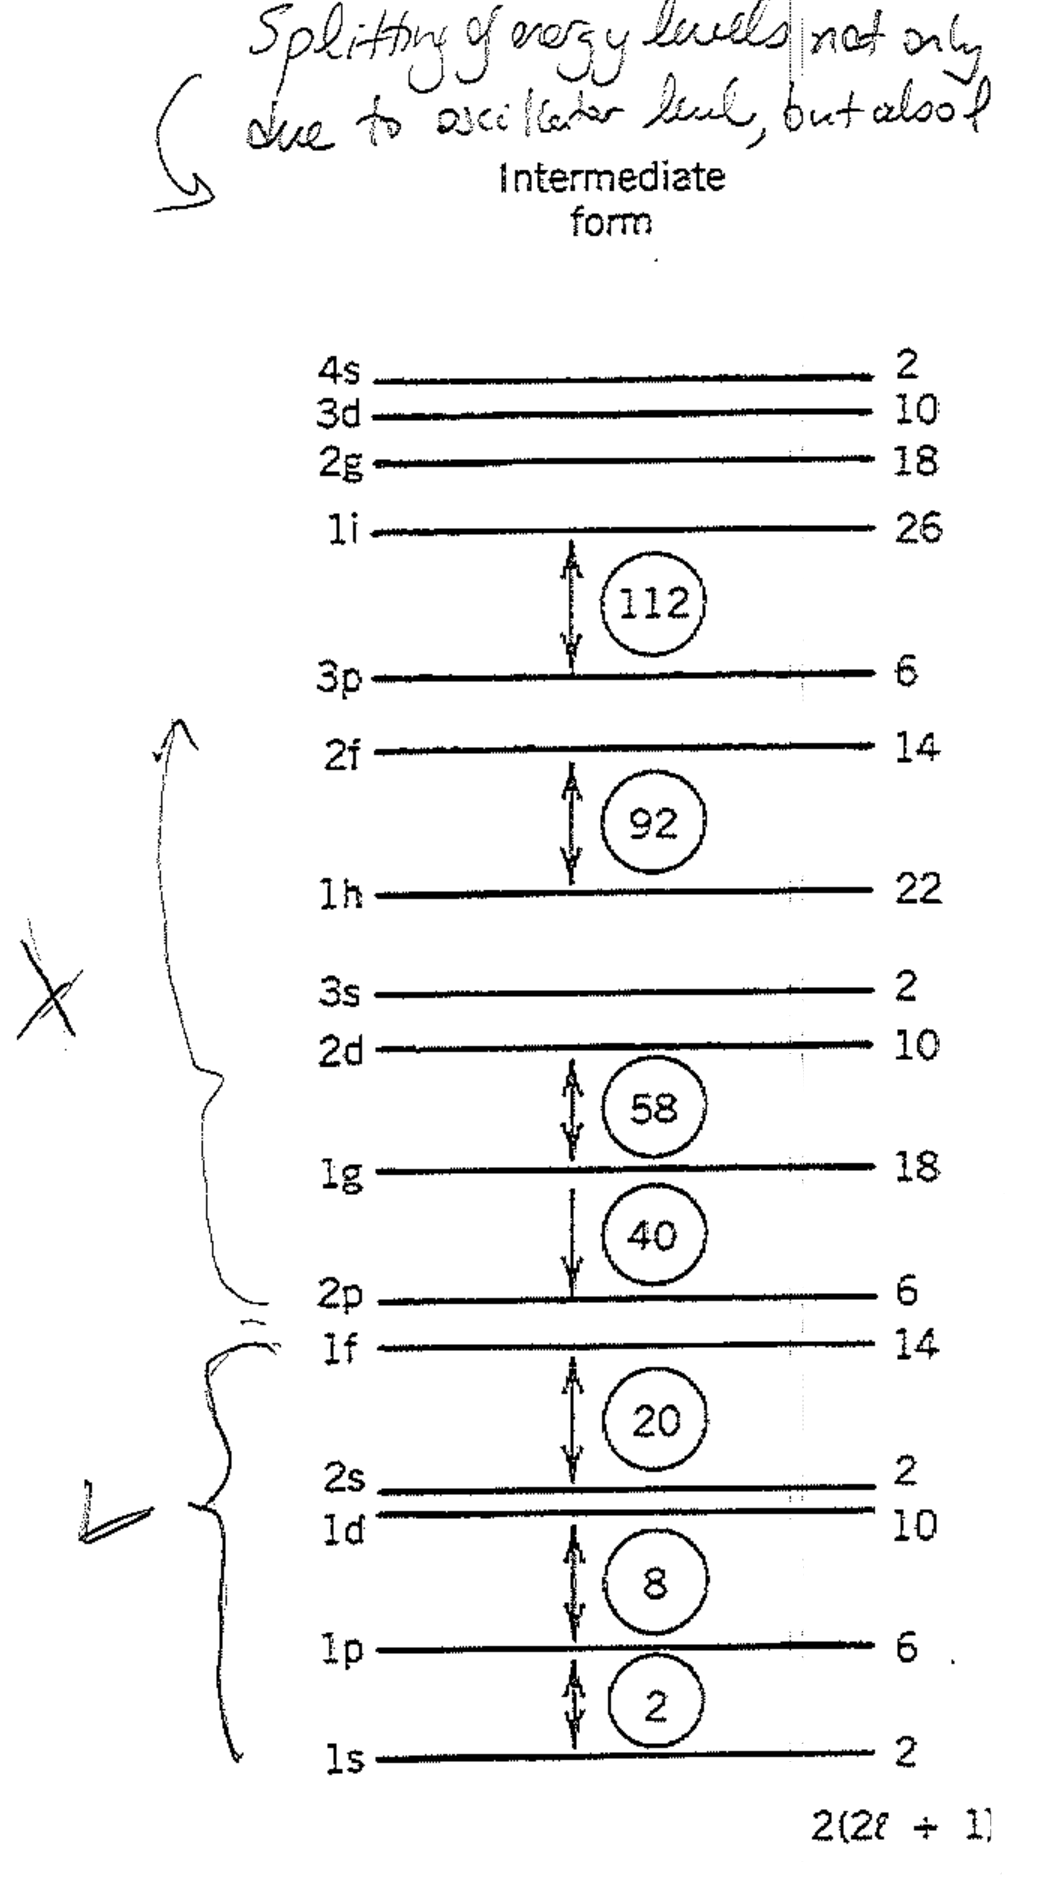
\includegraphics[width=2in]{images/shell/intermediate-potential-energy.png}
    \caption{Intermediate Form Energy Level Diagram, Krane Figure 5,6 (a)}
    \label{intermediate-energy}
\end{figure}



\end{document}
